\documentclass[11pt]{article}
\usepackage[brazilian]{babel}
\usepackage[utf8]{inputenc} %acentuação da língua portuguesa
\usepackage[T1]{fontenc} 
\usepackage{wrapfig} %figura ao lado do texto
\usepackage{graphicx} %pacote de figuras

\usepackage{amsfonts} %pacote com \mathbb{}

\usepackage[pdftex]{hyperref} %links da internet

\usepackage{fancyhdr} 

\usepackage{hyphenat} %retirar hefenação

\tolerance=1 %retirar hefenação

\emergencystretch=\maxdimen %retirar hefenação

\hyphenpenalty=10000 %retirar hefenação

\hbadness=10000 %retirar hefenação

\hyphenchar\font=-1 %retirar hefenação

\sloppy %retirar hefenação

\usepackage{textcomp}

\usepackage[a4paper,left=2cm,right=2cm,top=2.5cm,bottom=2cm]{geometry}

\setlength{\parindent}{0pt} %Parágrafo sem identação]

\begin{document}
	
	\pagestyle{fancy}
	\renewcommand{\headrulewidth}{0pt}
	\renewcommand{\footrulewidth}{2.1pt}
	\fancyfoot[L]{\small Diego Silveira Costa Nascimento}
	\fancyfoot[R]{\small diego.nascimento@ifrn.edu.br}
	
	\begin{minipage}[c][1.5cm][c]{3cm}
		\begin{flushleft}
			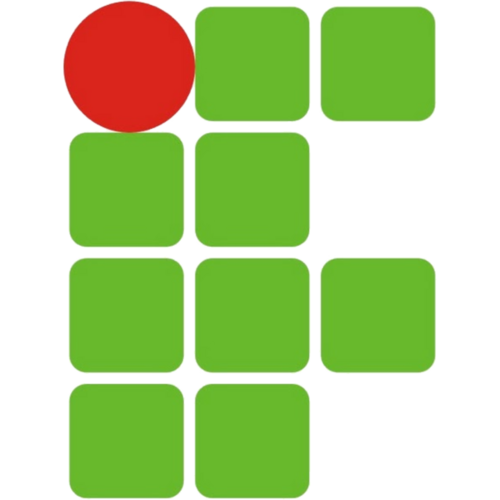
\includegraphics[scale=0.25]{IFRN}
		\end{flushleft}
	\end{minipage}		
	\begin{minipage}[c][1.5cm][c]{10.8cm}
		\begin{center}
			\resizebox{!}{0.3cm}{\textbf{Informática}}\par
			\resizebox{!}{0.2cm}{\textbf{Instituto Federal de Educação, Ciência e Tecnologia do Rio Grande do Norte}}\par
			\resizebox{!}{0.2cm}{\today}
		\end{center}
	\end{minipage}
	
	\begin{center}
		Exercícios
	\end{center}
	
	\section{História da Computa\c cão e Ergonomia}
	
	\begin{enumerate}
		\item Quais opera\c cões são possíveis de ser calculadas com o ábaco, e como é utilizado?
		\item Quais opera\c cões são possíveis de ser calculadas com o Bastões de Napier, e como é utilizado?
		\item Qual a precursora das calculadoras mecânicas, e qual opera\c cão é realizava?
		\item Quais os tipos de operações realizadas pela calculadora mecânica Leibnitz?
		\item Qual o componente utilizado no tear mecânico, que posteriormente foi utilizado para projetar máquinas de calcular?
		\item Quem é considerado o Pai da Computa\c cão, e por quê?
		\item Quais tipos de operações são realizadas pela Máquina Diferencial de Babbage?
		\item Quais as principais evoluções da Máquina Analítica de Babbage?
		\item Para que foi projetada a máquina de Tabula de Hollerith, e por quê?
		\item Para que ser um computômetro?
		\item Qual o primeiro computador a utilizar cálculos baseado em aritmética binária, e por quem foi desenvolvido?
		\item Para que foi projetado o Colossus?
		\item Qual o primeiro computador eletrônico digital de propósito geral, e suas características?
		\item Qual o primeiro computador comercial entregue a um cliente?
		\item O que é um mainframe?
		\item Qual o primeiro computador desenvolvido para fins pessoal, que trazia recursos como monitor e teclado?
		\item Qual o primeiro computador comercial a possuir interface gráfica e uso do mouse?
		\item Qual os objetivos em se preocupar com aspectos de ergonomia com o uso dos computadores?
		\item Descreva quais cuidados devemos ter ao utilizar o computador de forma ergonômica para: visão; punhos e bra\c cos; costa; e os pés.
	\end{enumerate}
	
	\newpage
	\section{Hardware}
	
	\begin{enumerate}
		\item O que é hardware?
		\item O que é um placa-mãe e sua finalidade?
		\item O que é um processador, em quais partes é organizado, e qual a fun\c cão de cada uma delas?
		\item Quais o tipos de memória, e para que serve cada uma delas?
		\item Quais o tipos de periféricos? Cite exemplos de cada um deles.
		\item Quais os tipos de impressoras? Cite quais são as vantagens e desvantagens de cada uma delas.
	\end{enumerate}

	\newpage
	\section{Software}
	
	\begin{enumerate}
		\item O que é software?
		\item O que é software de sistema? Cite exemplos.
		\item Quais as principais tarefas do software de sistema?
		\item O que é software de aplicativo?
		\item Quais os tipos de softwares aplicativos?
		\item O que é um software editor de texto, quais suas características? Cite exemplos.
		\item O que é um software editor de planilha eletrônica, quais suas características? Cite exemplos.
		\item O que é um software de produção, quais suas características? Cite exemplos.
		\item O que é um software de gerenciamento de informação pessoal, quais suas características? Cite exemplos.
		\item O que é um software de comunicação, quais suas características? Cite exemplos.
	\end{enumerate}
	
\end{document}